\begin{singlespacing}
\chapter{Data analysis and \atlas\ searches}
\label{chapter:searches}
\begin{epigraphs}
\qitem{%
One way is to make it so simple that there are \emph{obviously} no deficiencies
and the other way is to make it so complicated that there are no \emph{obvious}
deficiencies.%
}%
{Tony~Hoare,
\textit{The Emperor’s Old Clothes},
1981~\cite{hoare2007emperor}}
\end{epigraphs}
\end{singlespacing}

Our task in scientific data analysis is to distil an informative
message from data and to report that message to the wider community.
From any given data there are many possible messages that could be extracted,
and those messages will have different values to different recipients of our
messages --- our data analysis is not an automatic process, but a result
of many judgements that are informed by theory, convention, and intuition.

To clarify our later description of the $\twoljets$ search in
Chapter~\ref{chapter:2ljets}, this chapter introduces the basic theory and
practice of data analysis and its manifestations in the \atlas\ SUSY community.

Theoretical data analysis in the tightly coupled fields of probability theory
and decision theory is introduced in Section~\ref{sec:searches_data_analysis}.
An attempted alternative formulation, frequentist theory, is discussed in
Section~\ref{sec:searches_frequentist} for its relevance to our methods.
Standard practice in this field of research does not strictly follow
frequentist methods, but patches up some of their pathologies with modified
approaches that we describe in Section~\ref{sec:searches_practice}.
Searches for Supersymmetric signals in \atlas\ follow a standard strategy for
their data analysis; its procedures, nomenclature, and parametric modelling
are introduced in Section~\ref{sec:searches_searches}.


\section{Data analysis}
\label{sec:searches_data_analysis}
How many jelly beans are in the jar of Figure~\ref{fig:searches_beans}?
Your answer depends not only on what you observe from the figure, but also on
what else you know about cartoon jars of beans, and on what reward is on offer.
Each answer is a decision that depends both on what the possible rewards are,
and on which numbers of beans you subjectively infer to be likely.
We shall return to this example after developing some probability and decision
theory.

\begin{figure}[tp]
\centering
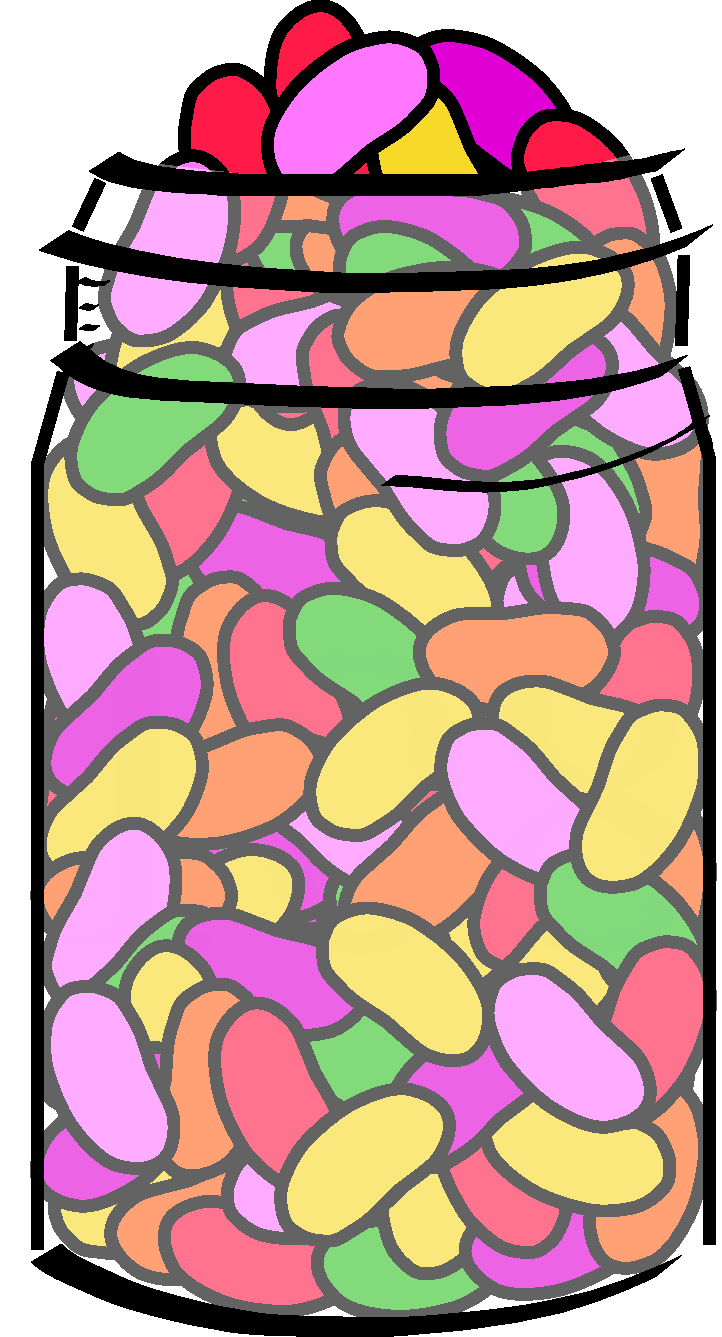
\includegraphics[width=0.25\textwidth]{figures/searches_beans.pdf}
\caption[
How many beans are in the jar?
]{%
How many beans are in the jar? This jar of jelly beans is a vehicle for our
discussion of inference and decision theory.
Please write your guess on this page.
The first correct answer wins a gold star.
}
\label{fig:searches_beans}
\end{figure}

Statistical data analysis suffers from dogma --- prescriptions and recipes that
students are taught to memorize and follow without knowing their reasons or
limitations.
From a standard undergraduate physics education, my experience has been
error propagation formulae,
least-squares fitting routines,
chi-squared per degree of freedom,
and myriad statistical tests and confidence intervals.
Many of these are effective approximations, but all also fail if misused
outside their domain.%
\footnote{%
Multiplicative error propagation is an example.
For $a = \mu_a \pm \sigma_a$ and $b = \mu_b \pm \sigma_b$,
the standard perturbative approximation is
\(
\widetilde{\sigma}_{ab}
= \mu_a \mu_b \sqrt{\sigma_a^2/\mu_a^2 + \sigma_b^2/\mu_b^2}
% = \sigma_a^2 \mu_b^2 + \sigma_b^2 \mu_a^2
\),
but a short calculation with their moments derives the exact result
\(
\sigma_{ab}
= \sqrt{(\mu_a^2 + \sigma_a^2)(\mu_b^2 + \sigma_b^2) - \mu_a^2\mu_b^2}
% = \sigma_a^2 \mu_b^2 + \sigma_b^2 \mu_a^2 + \sigma_a^2 \sigma_b^2
\)
if $a$ and $b$ are independent.
Since $\sigma_{ab}^2 = \widetilde{\sigma}_{ab}^2 + \sigma_a^2 \sigma_b^2$, this
propagation formula works only for small relative errors.
}
All effective methods of data analysis can be derived upwards from the roots of
probability and decision theory, and as elsewhere in physics, by knowing the
derivations we can also know when each approximation should work and when it
needs replacing.

We begin with what probability is: at its most abstract, a probability a
proportion of stuff within a larger whole.
Probabilities useful because proportions have applications, and because they
can be manipulated and interrelated with a linear and intuitive algebra.
Probabilistic data analysis follows the ordinary structure of science ---
write down models that make predictions, test those predictions against data,
then update your models to refine their predictions.
For this process, likelihoods are particularly important because they describe
our predictions. But not everything is a likelihood.
The remainder of this section uses a standard example from High Energy Physics
to introduce this probabilistic structure and other parts of its technical
language.

\subsection{Probability, abstract}
A probability $\prob{b}{a}$ is a number that quantifies the proportion
of $b$ within $a$, and can be expressed as a ratio~\cite{axioms1010038}
\begin{equation}
\label{eqn:searches_prob_ratio}
\prob{b}{a} = \frac{m(b, a)}{m(a)},
\end{equation}
in which $m(x)$ is a measure (a non-negative quantity assigned to its
argument, such as mass of tea in a cup), and the comma `,' means `and'
(logical and or set intersection or any other equivalent operation).
To continue that example, $\prob{b}{a}$ could be a proportion of tea within
a spoon within a cup, where $m(b, a)$ measures the volume of tea in a
teaspoon that is partially submerged in the cup.%
\footnote{%
All probabilities are conditional in this definition; $\probc{b}$ alone does
not exist unless some conditioning information is implicit from context.%
}

Logic is an important application of probability for which $a$ and $b$ are
interpreted as logical propositions, and
$\prob{b}{a}$ is the degree to which $a$ implies $b$, with the limiting cases
that $\prob{b}{a} = 1$ when $a$ implies $b$, and $\prob{b}{a} = 0$ when $a$
contradicts $b$.
Indeed, Cox's theorem derives the laws of probability by requiring compatibility
with Boolean logic~\cite{
cox1946probability,
cox1961algebra,
garrett1998nand,
jaynes2003probability,
keynes1920treatise
}.
Probability works for logic, and it works \emph{for tea, too}.

Two algebraic rules derive from Equation~\ref{eqn:searches_prob_ratio}:
a \textbf{product rule}
\begin{align}
\prob{c, b}{a} &= \prob{c}{b, a}\times \prob{b}{a},
\label{eqn:searches_product_rule}
\intertext{%
that describes nested proportions
(perhaps a spoon within a teacup within a sink),
and a \textbf{sum rule}%
}
\prob{c\vee b}{a} &= \prob{c}{a} + \prob{b}{a} - \prob{c, b}{a},
\label{eqn:searches_sum_rule}
\end{align}
that describes combination in a union $\vee$ that coincides with logical `or'.
The subtraction avoids double-counting of any overlap, and is often avoided by
splitting any problem into orthogonal, or disjoint states.
For disjoint cases with labels $b_i$, normalization therefore requires that
\begin{equation}
\label{eqn:searches_normalization}
\sum_i \prob{b_i}{a} = 1.
\end{equation}
These rules are basic and well known, but we state them here to support the
following statements of how probabilities can be applied for practical
results.%
\footnote{%
The formulation with sums and products is not strictly unique, but all
alternatives are equivalent up to an invertible
transformation~\cite{axioms1010038}.
This choice is usually best because it uses ordinary addition and
multiplication.
In numerical analysis, however, it is often practical to use $\log$
probabilities to avoid overflows outside the range representable by floating
point numbers, thus changing multiplication to addition and addition to
the `$\log$-add-$\exp$' operation.
}

\subsection{Probability, applied}
\begin{figure}[tp]
\centering
\begin{subfigure}{\textwidth}
\centering
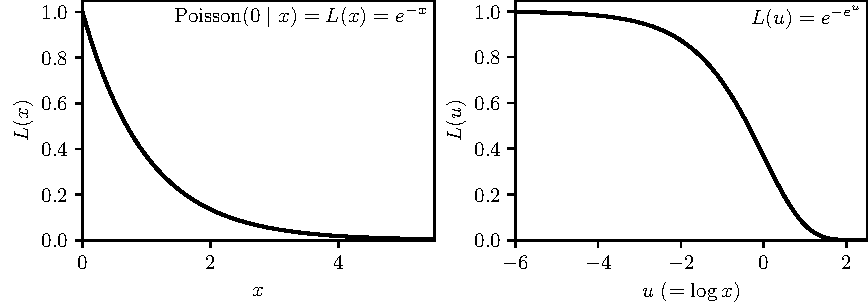
\includegraphics[width=\textwidth]{figures/searches_abacus_likelihood.pdf}
\caption{%
Likelihood: $\mathrm{Poisson}(0\mid x)$ in
(left) $x$ and
(right) $u = \log x$%
}
\end{subfigure}
\\[.5em]
\begin{subfigure}{\textwidth}
\centering
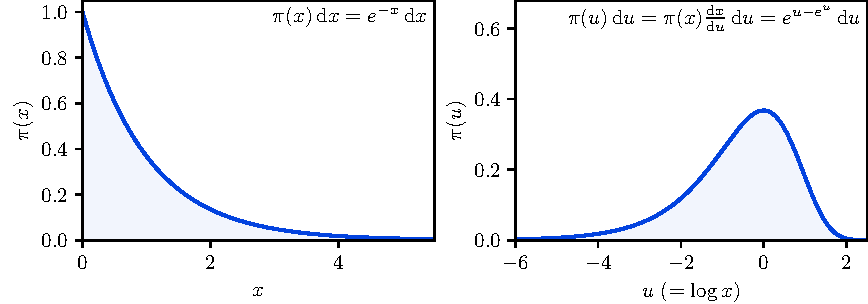
\includegraphics[width=\textwidth]{figures/searches_abacus_prior.pdf}
\caption{%
Prior density: exponential in
(left) $x$ and
(right) $u = \log x$%
}
\end{subfigure}
\caption[
Likelihoods and prior densities' different transformations
]{%
Likelihoods and prior densities' different transformations with coordinates.
The $\mathrm{Poisson}(0\mid x)$ likelihood and exponential $e^{-x}\mathrm{d}x$
prior have the same form, but the prior density changes to preserve its unit
area when expressed relative to $u = \log x$.
\\[.5em]
Relative to $x$, both are identical (left).
On changing to $\log$ coordinates (right), the likelihood slides horizontally,
but the prior density changes value to preserve area.
Both maximum likelihood points are equivalent (maximum likelihoods are robust),
but the maximum prior density moves (maximum densities are slippery).
\\[.5em]
Particle lifetimes follow exponential distributions, and their maximum
densities are at zero time.
It is misleading, however, to describe their most probable lifetimes as zero
---
the `most probable' $\log$ lifetime is not $\log 0$, but equals the mean
lifetime.
\\[.5em]
For zero Poisson data, the maximum likelihood rate is zero, but zero might not
be the most likely rate (if, for example, an experiment has known backgrounds).
}
\label{fig:searches_abacus}
\end{figure}
% science snake
Science involves making predictions, testing those predictions against data,
and reporting what is learned from the results.
Various probabilities are involved in this prediction and learning that have
conventional names to communicate what we intend to do with them.
Most important for prediction is a \textbf{likelihood}
\begin{align}
L(a) &= \prob{b}{a} \\
\label{eqn:searches_likelihood}
\intertext{%
that explores the probabilities assigned to a fixed result $b$ from different
contexts $a$, or how well different hypotheses predicted a result.
A likelihood is clearly a probability, but it is not a probability distribution
--- only the left hand argument $b$ forms a normalized distribution.
Alternatively, fixing the context gives a \textbf{prior}%
}
\pi(b) &= \prob{b}{a}
\label{eqn:searches_prior}
\end{align}
for fixed $a$, which is a normalized distribution over disjoint states $b$.

Since prior probabilities are normalized distributions, it is usually
convenient to represent them as density functions.
Densities are stated relative to coordinates (or occasionally measures),
so changing coordinates changes their values as their unit probability mass
is sloshed around.
Likelihoods are not densities in the conditioning variable that they explore,
so changing coordinates slides them horizontally like beads on an abacus,
but does not change their values for equivalent states.
Figure~\ref{fig:searches_abacus} illustrates this difference.

Likelihood and prior are evidently related --- they explore two indices into
the same object, two sides of the same coin, and are assigned by the same
principles.
But they are profoundly different objects that work for different purposes,
and clarity in their distinction will help in our later understanding of
practical methods.
We use likelihoods to compare which hypotheses predicted observed data better
than others.
Prior to observing data we use priors to describe what might result from
different models; priors on data can be useful in designing our experiments,
and priors on other states describe other predictions.

To illustrate this, consider a histogram that bins event yields in
$\met$, with distributions from background and (supersymmetric) signal samples
overlaid.
Example such histograms are displayed in
Figure~\ref{fig:searches_sig_bkg_prior_likelihood}.
Since these histograms are normalized to unit area, they show prior
probability distributions along the bin axis; there is one prior
for events from each of the background and signal hypotheses.
Priors distribute unit probability explore along the bin axis.
In each bin, however, a likelihood function compares the assignments from
the two hypotheses: signal and background.
Likelihoods explore vertically down the sample axis.

\begin{figure}[tp]
\centering
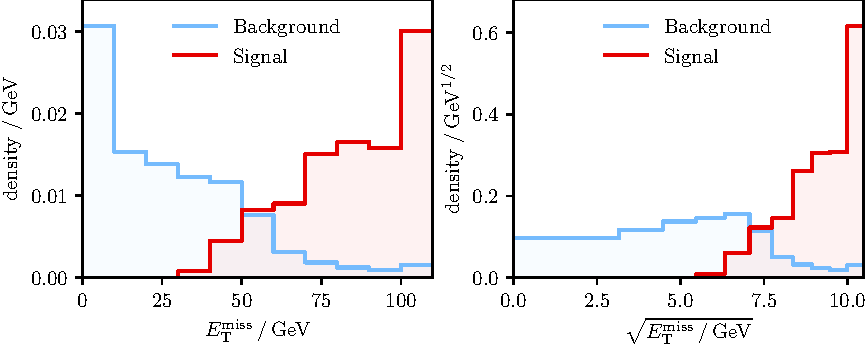
\includegraphics[width=\textwidth]{figures/searches_sig_bkg_prior_likelihood.pdf}
\caption[
Background and signal prior densities
]{%
Background and signal prior densities in $\eV[G]$ and $\eV[G]^{1/2}$ units.
When changing coordinates, probability mass moves as a fluid of constant total
volume, changing its shape in this density view to keep the area of the
rectangle in each bin constant.
A likelihood function indexes each bin in the background--signal labels,
and is independent of the coordinates units since the area in each bin is
invariant.
}
\label{fig:searches_sig_bkg_prior_likelihood}
\end{figure}

Identical distributions are drawn in two different coordinates
on the left and right of Figure~\ref{fig:searches_sig_bkg_prior_likelihood};
they are identical in content, but differ in appearance because they use the
standard approach of representing each prior distribution as a density.%
\footnote{%
Density is a somewhat misleading term here.
Probability mass does not compress, it moves and redistributes --- it is more
like depth of tea than density of air.%
}
To preserve the area of each bin, which shows its probability mass,
bin heights therefore change to adapt to their widths that change due to the
differing values of $\met$ and $\sqrt{\met}$.
This coordinate-dependence of the prior density means that its maximum is
not always meaningful.
Since the probability mass in each bin is constant, the likelihood is
coordinate-independent.

One typically approximates such histograms by Monte Carlo simulation methods,
since simulations do not generate bin indices but event variables that derive
from the sampled events.
To connect these concept with probabilities, we begin with some notation;
we have hypotheses $h$ (signal or background),
a parameter $x$ that we histogram ($x = \met$),
and we observe a datum $d$ that datum indexes the histogram bins --- supposing
an event is observed in the overflow bin, it says
$d = `x > 100\,\eV[G]\textrm{'}$.
This observed bin has a likelihood function
\begin{equation}
L(x) = \prob{d}{x, h} = \prob{d}{x} =
\left\{
\begin{matrix}
1 & \textrm{if }~x > 100\,\eV[G], \\
0 & \textrm{otherwise} \\
\end{matrix}
\right.
\end{equation}
that corresponds to Equation~\ref{eqn:searches_likelihood} by
$b \leftarrow d$ and $a \leftarrow `x, h\textrm{'}$,
and simplifies $\prob{d}{x, h} = \prob{d}{x}$ since such binning is independent
of hypothesis.%
\footnote{%
Independence of the likelihood function from prior hypotheses is so common
that it should usually be assumed unless otherwise stated.
}
This example of a binary selection highlights how the likelihood acts as a
filter that rejects events that are contradicted by the data.
Other likelihoods that are not binary act similarly, but as inefficient filters
that reject events with some probability.

Simulating events from background and signal hypotheses samples from their
respective priors
\begin{equation}
\pi(x) = \prob{x}{h}
\end{equation}
that correspond to Equation~\ref{eqn:searches_prior} by
$b \leftarrow x$ and $a \leftarrow h$.
Although we previously used the same labels $a$ and $b$, those are only
labels --- the words `prior' and `likelihood' state our intent to index into
the left and right arguments, respectively.

When we fill a histogram by summing weights of simulated samples, we are
calculating another likelihood over hypotheses $h$ alone, not $`x, h\textrm{'}$
jointly.
To disambiguate the two, we call this abstracted, $x$-independent likelihood
the \textbf{evidence} $Z(h)$ for hypothesis $h$.
The evidence is calculable as
\begin{align}
Z
= \prob{d}{h} &= \sum_i L(x_i) \,\pi(x_i)
\label{eqn:searches_evidence_integral_sum}
\\
&= \int\! L(x) \,\mathrm{d}\pi(x),
\label{eqn:searches_evidence_integral_measure}
\end{align}
where Equation~\ref{eqn:searches_evidence_integral_measure} is notation for
integrating the likelihood function over the prior measure~\cite{
billingsley2008probability,
skilling2010foundations
}, and relates most closely to our practice of simulating from the model and
counting events that hit the non-zero likelihood in the bin.
We shall shortly derive this identity.
The name `evidence' relates to its application for model
comparison~\cite{mackay2003information}.
Supposing we have this one event with $\met > 100\,\eV[G]$, did it come from
the background or signal sample?
The answer depends on the signal and background cross-sections in our collider,
but larger evidence for signal does influence any conclusion to move in its
favour.

This expression as an integral --- an average over the prior, means that
the evidence $Z$ depends on what fraction of samples hits large values of
the likelihood function, and not only on how large that likelihood gets.
In contrast, one could consider a maximum likelihood approach that would
constrain a numerical optimization to regions of non-zero prior in each model.
Such optimizations can give useful upper bounds on the evidence, but this
example highlights a flaw when both models support the $\met > 100\,\eV[G]$
bin.
Then, both support the same maximum likelihood of
$L(\varepsilon + 100\,\eV[G]) = 1$, despite different evidence values.

% posterior
Perhaps we now want to see where in the overflow bin this event landed, and
compare the signal and background distributions there.
This is an inspection of the \textbf{posterior}
\begin{equation}
p(x) = \prob{x}{d, h} = \frac{L(x)\,\pi(x)}{Z},
\end{equation}
which is a prior probability distribution specialized by the data;
it simply uses the likelihood to filter simulated samples
(perhaps in `skimming an ntuple')
and re-normalizes them to a probability distribution within the constraint.

We finally have the four parts of `Bayesian' data analysis:
the two inputs \textbf{likelihood} and \textbf{prior},
and two outputs \textbf{posterior} and \textbf{evidence}.
These relate through Bayes' rule, which is a consequence of the
produce rule of Equation~\ref{eqn:searches_product_rule} and the
commutativity of `and' --- that `$a$ and $b$' is equivalent to
`$b$ and $a$';
the joint probability of data and parameters has two identical
forms, $\prob{d, x}{h}$ and $\prob{x, d}{h}$, that each factor into two
pieces:
\begin{align}
\prob{d}{x, h}\times \prob{x}{h} &= \prob{x}{d, h}\times \prob{d}{h},
\intertext{all of which we have named:}
\underbrace{L(x)}_\textbf{likelihood}
\times
~\,
\overbrace{\pi(x)}^\textbf{prior}
~\,
&=
\overbrace{p(x)}^\textbf{posterior}
\times
\underbrace{Z}_\textbf{evidence}
.
% \textbf{likelihood} \times \textbf{prior}
% &= \textbf{posterior} \times \textbf{evidence} .\nonumber
\end{align}
This is (the infamous) Bayes' rule, derived as a consequence of the
symmetry of logical `and' and the product rule of probability
algebra.

How Bayes' rule \emph{should} be used in scientific data analysis is to extract
useful information from the data.
If the likelihood function itself is interpretable, then it should be reported
directly.
When it is not, perhaps due to a complicated parametric modelling, then one
should abstract those parameters away to summarize the likelihood.
Properties such as local maxima or regions in which it exceeds meaningful
thresholds can be useful.
Evidence values for predictive models can also be useful if those models are
clearly stated and relevant to readers' interests.
Data act only through the likelihood function, and reporting a posterior
can act to obfuscate those data.

Posterior probabilities are, however, useful when digesting data to make
inferences about the world.
Reporting likelihood functions and evidence values allows readers to assign
priors as they wish.
For model comparison, for example between background $h=B$ and signal $h=S$
models, the analysis is conveniently linearized by expressing it in $\log$
ratio form:
\begin{equation}
\hphantom{\quad \quad \mid\mid \mathrm{context}}
\phi(d) =
\log\frac{\prob{S}{d}}{\prob{B}{d}}
=
\log\frac{\prob{d}{S}}{\prob{d}{B}}
+
\log\frac{\probc{S}}{\probc{B}}
\quad \quad \mid\mid \mathrm{context}
,
\end{equation}
where we use the double bar, $\mid\mid$, to refer to any contextual information
a reader might wish to include.
When the evidence ratio is independent of that context, as it usually is,
it factors out from the prior (odds) ratio.
In this sense, likelihood (or evidence) ratios are scale factors that update
any odds prior ratio by the same multiplication, and that on this $\log$ scale
that means just adding a constant.

From such $\log$ ratios one individual probabilities are recovered through the
logistic function:
\begin{equation}
\label{eqn:searches_logistic}
\prob{S}{d} = \frac{1}{1 + e^{-\phi(d)}}
.
\end{equation}
Physically, this is analogous to the Boltzmann distribution where the energy
of each model is its negative $\log$ probability, with unit inverse
temperature~\cite{
pmlr-v2-ranzato07a,
skilling2017david
}.
With multiple models in play, it is also called the `softmax'
function~\cite{MurphyKevinP.2012Mlap}.

The infamy of Bayes' rule stems from a fixation on the posterior distributions
from unjustified prior assignments.
Classical works by
Bayes~\cite{bayes1763lii} and
Laplace~\cite{laplace1774stigler} began this focus ---
both assume prior densities that are uniform in chosen coordinates, a practice
that can yield practical results in posterior inferences.
But to report scientific data, such practices are fairly criticized as
arbitrary when they influence the reported results.
Prior assignments are arbitrary.
You are welcome to propose any prediction in any circumstances, and the
scientific response is to test whether or not its predictions are compatible
with our observations of nature.
Our emphasis on the likelihood functions and evidence values that quantify
those predictions avoids the pitfall of seeking uninformative, neutral, or
unbiased priors by embracing priors as active and explicit predictions.
This is the modern, practical approach to Bayesian data analysis~\cite{
mackay2003information,
skilling2004nested,
skilling2006nested,
sivia2006data,
skilling2010foundations
}.

\begin{figure}[tp]
\centering
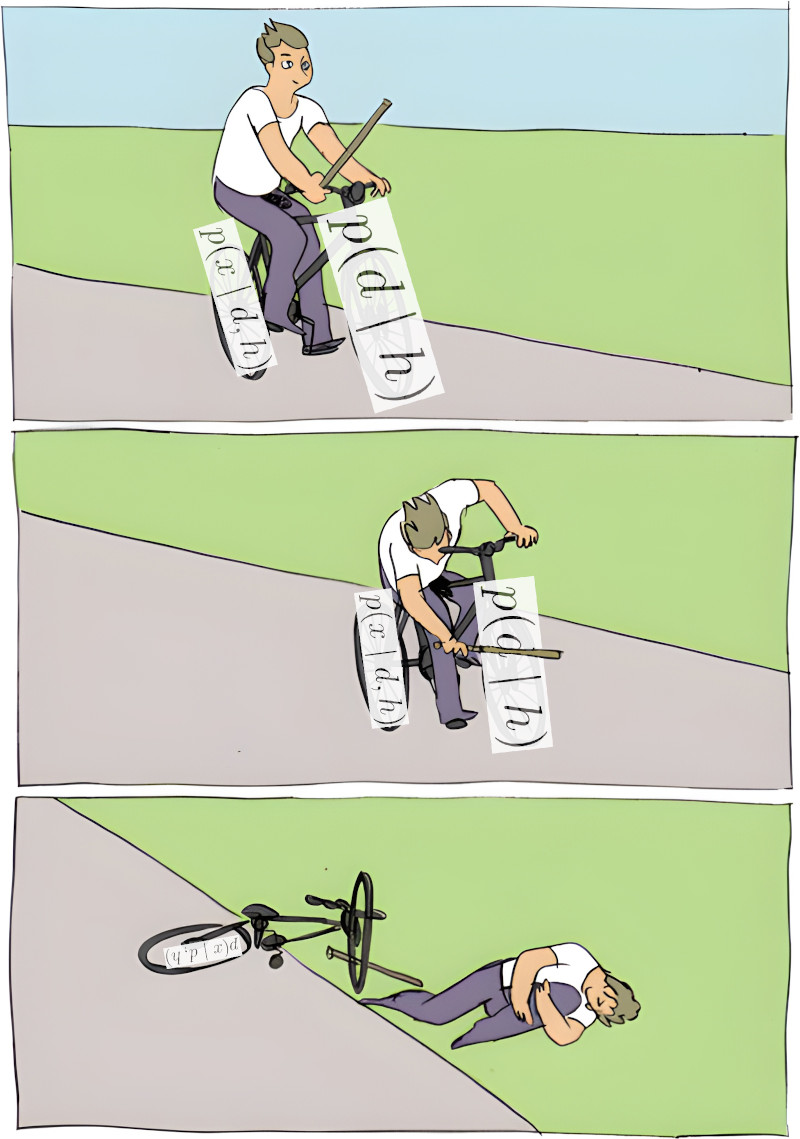
\includegraphics[width=0.65\textwidth]{figures/searches_baton_roue_bayes.jpg}
\caption[
Bayesian analysis produces two outputs: the evidence and posterior
]{%
Bayesian analysis produces two outputs: the
evidence $\prob{d}{h}$ and
posterior $\prob{x}{d,h}$ for hypothesis $h$, data $d$, and parameters $x$.
Posterior-only, semi-Bayesian methods are legitimately criticized because they
do not challenge the hypotheses that assign their priors $\prob{x}{h}$.
Since the evidence is a likelihood function over hypotheses, considering the
evidence can challenge those priors.
\\[0.5em]
Cartoon adapted from ``Baton roue'' by
Corentin~Penloup~\cite{penloup2011baton}.
}
\label{fig:searches_baton_roue_bayes}
\end{figure}

Some sources continue to define Bayesian analysis as the computation of
posterior probabilities given data, often without naming the evidence, and
expressing it only as the sum from
Equation~\ref{eqn:searches_evidence_integral_sum}
--- as just a normalizing constant~\cite{
gelman1995bayesian,
gelman2008objections,
DAgostini:1994fjx,
DAgostini:2010hil,
cowan1998statistical,
pdg2020review
}.
Bayes' rule has two outputs, and both outputs have uses.
Cutting out the evidence hamstrings Bayesian analysis, leaving only the
semi-Bayesian posterior-only approach and its clear flaws.
A bicycle is stable with two wheels and falls over if one either
is removed;
Figure~\ref{fig:searches_baton_roue_bayes} illustrates this analogy.
Although it is possible to ride a unicycle, it is a circus trick and not often
a practical tool.

Phrased succinctly by Skilling~\cite{skilling2008rant},
``we SHOULD use Bayes by assigning subjective priors and inspecting evidence
values.''
This framing of probabilistic data analysis agrees exactly with our standard
practice of histogramming simulations,
as illustrated in Figure~\ref{fig:searches_sig_bkg_prior_likelihood}:
signal and background models define priors, and their (normalized) bin yields
are the evidence values that we use to compare the models.
Finally, their corresponding posteriors are the normalized shapes those samples
take within the observed histogram bin, with which we do not compare the
models, but which could in principle be used for secondary interpretations.

\subsection{Probability assignments}
Probability algebra manipulates probabilities, but does not state how they
should be initially assigned.
In general, such probability assignments are free and unconstrained, and might
be informed by calibration data or loosely motivated opinions.
But there are examples of unambiguously derived that are commonly used in
High-Energy Physics, notably the Poisson and Gaussian distributions.
To avoid turning this thesis into a textbook, we only sketch the derivations
of these, and refer to real textbooks for their detailed
derivations~\cite{jaynes2003probability}, both of which use the exponential
identity that
\begin{equation}
\label{eqn:searches_exponential}
\exp(x) = \displaystyle \lim_{N \to \infty}
\left(1 - \frac{x}{N}\right)^N
.
\end{equation}

The Large Hadron Collider collides $40$~million proton bunches per second,
but \atlas' trigger system accepts only around $1000$ of
those per second~\cite{atlas2020trigger}.
This means that we have a scenario with a large fixed number $N$ of trials
(bunch collisions)
and a small probability of binary acceptance (triggering),
due to a notable collision event.
The summed total number $n$ of accepted events is therefore described by the
binomial distribution for $n$;
\begin{equation}
\label{eqn:searches_binomial}
\mathrm{binomial}(n\mid N, p) = p^n (1 - p)^{N - n} \times \binom{N}{n}
,
\end{equation}
which is a product of the probabilities (produce rule) in the sequence of $N$
accept/reject decisions, summed (sum rule) over all permutations of that sequence
that could have led to the total $n$.
With our tiny trigger rate, we are interested in the limit of small
$p$ and large $N$, which result in a mean acceptance number of $\lambda = Np$.
Using the exponential identity of Equation~\ref{eqn:searches_exponential}, one
can show that this limit tends towards the Poisson
distribution~\cite{jaynes2003probability};
\begin{equation}
\label{eqn:searches_poisson}
\mathrm{Poisson}(n\mid \lambda) = \frac{\lambda^n}{n!}\exp(-\lambda)
,
\end{equation}
which is used ubiquitously in the analysis of our histograms.

The Gaussian distribution has many justifications:
as the unique distribution that is spherically symmetric and factors linearly
into independent dimensions~\cite{
jaynes2003probability,
herschel1850normal,
maxwell1860normal,
muller1959note,
marsaglia1972normal
},
as a practical approximation that permits analysis in linear algebra,
and as the maximum entropy~\cite{PhysRev.106.620} distribution for a
known mean and variance.
This maximum entropy statement means that for a distribution with known mean
and variance in given coordinates, its best Gaussian approximation matches
those moments.\footnote{%
By `best', this statement means a minimal Kullback-Leibler divergence
\(
H(p\leftarrow q) = \sum_i p_i \log(p_i/q_i)
\)
from the Gaussian approximation $q$ to the target $p$ with known moments.
Such an approximation may not be \emph{good}, but it is best in class.%
}
As a limiting approximation, the Gaussian form arises from products of many
functions, such as combinations of many independent measurements that multiply
their likelihood functions.
At a maximum $\check{x}$, the first derivative of a function vanishes and the
second derivative is negative.
Taylor expanding about this maximum to the leading order, the product looks like
\begin{equation}
f(x)^N = \displaystyle \lim_{N \to \infty}
\left(
1 - \kappa (x - \check{x})^2
\right)^N,
\end{equation}
which, again by Equation~\ref{eqn:searches_exponential}, goes into the Gaussian
form
\begin{equation}
\label{eqn:searches_gaussian}
\mathrm{Gaussian}(x\mid \mu, \sigma)
\,\mathrm{d}x =
\frac{1}{\sqrt{2\pi \sigma^2}}
\exp\!\left(-\frac{1}{2}\frac{(x - \mu)^2}{\sigma^2}\right)
\mathrm{d}x
\end{equation}
where the prefactor is for normalization to a probability distribution over
$x$, and we include the $\mathrm{d}x$ terms as reminders that it is a density
function in $x$, not a probability exactly.
On a $\log$ scale, the Gaussian form is simply quadratic in $\mu$ (or $x$);
that quadratic form continues in its multivariate generalization, and
justifies least-squares methods.

Here, $\kappa$ and $\sigma$ both relate to the second derivative of the target
function; this relationship extends to multiple dimensions in the Hessian
matrix and its inverse, and allows one to estimate error bars from second
derivatives --- a practical tool that the methods discussed in this thesis
employ.

This is not the famous Central Limit Theorem, which is related to the
distribution of sums.
But can be used to derive it: the distribution of a sum is a convolution, which
becomes a product in Fourier-transformed space, and that product can converge
to a Gaussian function by this same derivation if the mean and variance exist.
A beautiful alternative proof of the Central Limit Theorem is given by
Jaynes~\cite{jaynes2003probability}
(Section ``7.16 The central limit theorem''), but would be spoiled by a
reproduction here.

In the current year, it would be remiss to not mention machine learning
algorithms.
Among various other applications, learning algorithms demonstrate practical
successes in probability assignments, such as assigning
probabilities to labels for classification,
or to assign probabilities to words for text
generation, or any of myriad other
predictions~\cite{MurphyKevinP.2012Mlap, radford2019language}.
Machine learning tunes flexible functions by consuming data and testing their
predictions in the manner we have described; their training and testing works
roughly as follows:
\begin{enumerate}
\item Predict new data with $\prob{d_i}{f(d_{i-1}, \ldots), h}$.
Keep this evidence as a testing score for comparison against other models.
(Practically, keep its equivalent $\log$ mean over independent samples.)
These $d_i$ may be only reductions of the data, such as class labels
or index permutations~\cite{Noroozi2016jigsaw, multitaskself2017}.
Other inputs that are not predicted, such as associated images that the machine
uses to predict the labels, are included in the context $h$.
\item Use those data to update your state
$f(d_{i-1}, \ldots) \rightarrow f(d_i, d_{i-1}, \ldots)$.
Unlike ideal posterior updating, this encodes only a function of the data, not
its whole --- one usually cannot afford to consume all aspects of data, so
although theoretically suboptimal this approximation is vastly superior in
practice.
Learning only part of the data is not wrong, it is just less precise than a
divinely perfect learning algorithm, which we do not currently possess.
\item Go to 1.
\end{enumerate}
These sequential data $d_i$ might be labelled the `training', `validation',
and `testing' sets, but other splittings are possible.
This perspective highlights the importance of independent training and testing
sets --- since $\prob{d}{d, \ldots} = 1$, if any memory of $d_i$ is kept in
the $f(\ldots, d_i, \ldots)$ state, then it is a memory and not a prediction.
Independent testing data permit the evidence interpretation of predictive
probabilities.


\subsection{Decision theory}
Now that we have thoroughly covered probability theory, we are ready to return
to the jelly bean game that is illustrated in Figure~\ref{fig:searches_beans}
and asks you to guess how many beans are in the jar.
Given all you know about illustrations of jars and beans, you could make a
vague guess without looking.
That guess should only be refined after inspecting the image and updating your
model to account for it.
Although I do not propose that human brains \emph{do} use probability
algebra~\cite{jaynes1988brain}, this inference process could, in principle,
be modelled numerically by distributing probability over the positive integers
and updating those probabilities in light of a likelihood function for the
image data.
Any guess, however, does not depend only on that probability distribution,
but on the risks and rewards associated with guessing.

As written in the caption to Figure~\ref{fig:searches_beans}, there is a
notional reward to the first exactly answer.
You are therefore incentivized to answer a) quickly, before other good guesses,
and b) exactly, with no reward for being close to the true answer.
If you are the first to answer, then it makes sense to write what you think
is the most probable number.
But others following you, seeing your answer, should prefer to guess
differently if they want to win (and they think any other guess is plausibly
correct).

To try hard, you could even dissect the vector graphics of the figure and count
its bean objects, but that may not be optimal use of your resources --- the
dubious promise of a gold star may be worth little to you.

When considering what decision to make, it feels natural to consider what
might result from each possible action and to judge that action on how good or
bad its results would be.
Mathematical decision theory agrees with this intuition---
a famous theorem by Wald~\cite{
wald1947bayes,
wald1950bayes,
jaynes2003probability
}
shows that the optimal solution to any decision problem can be always be
formulated as the minimization of an expected cost function, or risk:
\begin{equation}
\label{eqn:searches_bayes_decision_rule}
R(t) = \int\! c(t, x) \,\mathrm{d}p(x)
,
\end{equation}
where we mean `expected' in the mathematical mean sense of the `mean' average.
This cost function $c(t, x)$ evaluates the badness of outcomes for a given
decision $t$ and states of the world $x$ to which context must assign prior
probabilities $p(x)$.
For a given cost function and prior, one should choose the decision $t$ that
minimizes $R(t)$.

Although alternative ideas (such as minimax, minimizing a maximum
loss~\cite{savage1951review}) can work well in certain contexts, this theorem
states that restricting oneself to minimizing an expected cost function cannot
deny one access to optimal decisions.
Alternative formulations can at best be equivalent.

This theory does not, however, define how to construct that cost function.
Like the prior, it must come from context, and indeed the two are intertwined
in the risk;
decision-making machines and organisms are capable of learning to make good
decisions without constructing either cost or prior explicitly.
Towards our goal of usefully reporting data, such decision theory has been
applied to argue for ways to quote properties of posterior distributions.
As examples, minimizing the expected absolute error $|x - \check{x}|$ leads
to reporting the median, and minimizing the expected square error
$(x - \check{x})^2$ leads to reporting the mean.
Had the rules of our bean counting game rewarded you based on such distances,
these results could have been good guesses. But those weren't the rules.

When arguing that we should report likelihoods and evidence values for our
data, we have not explicitly constructed cost functions, nor have we made
quantitative predictions of future events.
But we can qualitatively consider them in this decision theory framework ---
we imagine that future scientists will want to reuse our data, and would be
pleased (attain a small cost) if they were able to reinterpret the results for
their own models.
We can therefore reason that likelihoods would usually have more utility than
alternatives such as point posterior averages.

% connection to frequentist section
An amusing feature of Wald's theory is that it was formulated from a
perspective on probability in which,
``In most applications, however, not even the existence of an a priori
distribution can be postulated''~\cite{wald1950bayes}.
That might seem problematic, since the risk is the expectation value of a cost
function over a prior (or \emph{a priori}) distribution.
Wald was nonetheless interested in these decision rules for their
``completeness'' that he had proven, and named them ``Bayes'' decision rules
despite approaching the theory from a stalwart non-Bayesian perspective.

Although Bayes' rule is not seriously disputed, the system in which Wald was
working defined probability as a frequency in random sampling, which cannot
reasonably apply to subjective, non-random distributions of probability mass
that many prior distributions are.
This frequency-restricted, `frequentist', philosophy dominated 20th century
statistical research, and influences practices that \atlas\ continues to
employ.
We therefore review some features of frequentist statistics in the following
section.

\begin{singlespacing}
\section{Frequentist theory}
\label{sec:searches_frequentist}
\begin{epigraphs}
\qitem{%
Within this theory, statistical methods of great practical usefulness have been
developed, and its statements can and frequently do contribute in a vague way
to the interpretation of data. \ldots%
}%
{John~W.~Pratt,
\textit{Review: Testing Statistical Hypotheses},
1961~\cite{pratt1961testing}}
\end{epigraphs}
\end{singlespacing}

Probability as defined in Equation~\ref{eqn:searches_prob_ratio} is a
proportion of stuff within a larger whole, which when formalized as a ratio
of measures and has broad applications.
Frequentist theory confines itself to the special case where those measures
are numbers of discrete randomly occurring events, such that a frequentist
probability is a ratio of frequencies:
\begin{equation}
\label{eqn:searches_prob_frequency_ratio}
\freq{b}{a} = \lim_{N \to \infty}\frac{n}{N},
\end{equation}
where $n$ is the number observed to satisfy conditions $a$ and $b$ when
$N$ have satisfied $b$.
Interpreted with the Binomial model of
Equation~\ref{eqn:searches_binomial}, this definition converges to our more
general probability whenever it applies.

We do think of many processes as random when considering scientific data, so
this definition works widely for likelihood functions.
Non-data hypotheses, however, are rarely considered as actually random events,
so the frequency definition cannot not apply.
Prior predictions often apply probabilities to express a subjective uncertainty
predictions that are manifestly non-random.
Under this frequency definition, those predictive probabilities are nonsense
and must be rejected.
The frequency definition does not change probability algebra, it only restricts
it to a permitted scope.

Coin tosses, for example, can be imagined as random.
Earth's human population could toss a few billion coins to precisely
establish a probability of landing heads from the ratio of
$n$ (number of heads) to $N$ (number of tosses).
But suppose you are given a red envelope containing a coin ---
which way up is the coin in the envelope?
You could guess or bet on the answer, and that decision might involve a tacitly
assumed probability.
A frequency, however, would only be permitted if the envelope had been packaged
randomly.
Was the coin first tossed to randomize its face, or placed deliberately?
It is unclear.

Tom Stoppard's play `Rosencrantz and Guildenstern Are Dead'~\cite{
stoppard1967rosencrantz
}
contains a clearer example ---
Rosencrantz and Guildenstern toss a coin ninety-two times, all landing heads
(by ``un-, sub- or supernatural forces'').
They play a game with a third player, landing eight more heads.
Is the next toss heads or tails?
The answer is not random --- it is burned in print onto paper, so no frequency
can be assigned.
Were subjective probabilities permitted, you could predict the result, and that
prediction would be subjectively informed by it being the one-hundred-and-first
toss, our cultural entanglement with round numbers in base-10, and your reading
of these words.
Frequentist theory, however, forbids such subjective probabilities of
non-random unknowns, so is left seeking alternatives.

As established in Section~\ref{sec:searches_data_analysis}, the original
probability theory of Laplace and Bayes, did not require frequency
interpretations; these were developed later in the 19th century by
mathematicians including Venn~\cite{venn1866logic} and
Boole~\cite{boole1854investigation}, in reactions that may well have been
propelled by reasonable objections to flawed posterior-only methods.
Modern frequentist theory has a rigorous set-theoretic formulation in the
Kolmogorov axioms~\cite{
kolomogoroff1933de,
kolomogoroff1950translated,
axioms1010038
}.
Applied frequentist methods, unlike frequentist theory, are constrained with
considerably less precision --- the denial of certain (non-frequency)
probabilities does not construct their replacements, and various surrogates
have evolved.
Modern frequentist methods are largely attributable to the authors
R. A. Fisher (for likelihood, $p$-values, and estimation criteria), and
J. Neyman and E. S. Pearson
(for statistical hypothesis testing and confidence intervals).
Together these do not form a harmonious or consistent framework ---
the two groups have emphatic disagreements in print ---
but do cover many practices that continue to survive in modern science
and explain important features of the methods apply to LHC data, which will be
introduced in Section~\ref{sec:searches_practice}.



\TODO{Fisher's great contribution --- likelihood}
\TODO{
Fisher:
criteria for estimators,
(consistency, efficiency, sufficiency)
~\cite{fisher1922estimators}
testing, p-value,
likelihood, also ratios of p-values (here named probable errors)
(introduced the term likelihood? cite?)
~\cite{fisher1921probable}
tail area = significance
~\cite{fisher1925smrw}
}
Figure~\ref{fig:searches_fisher_likelihood}


\begin{figure}[tp]
\centering
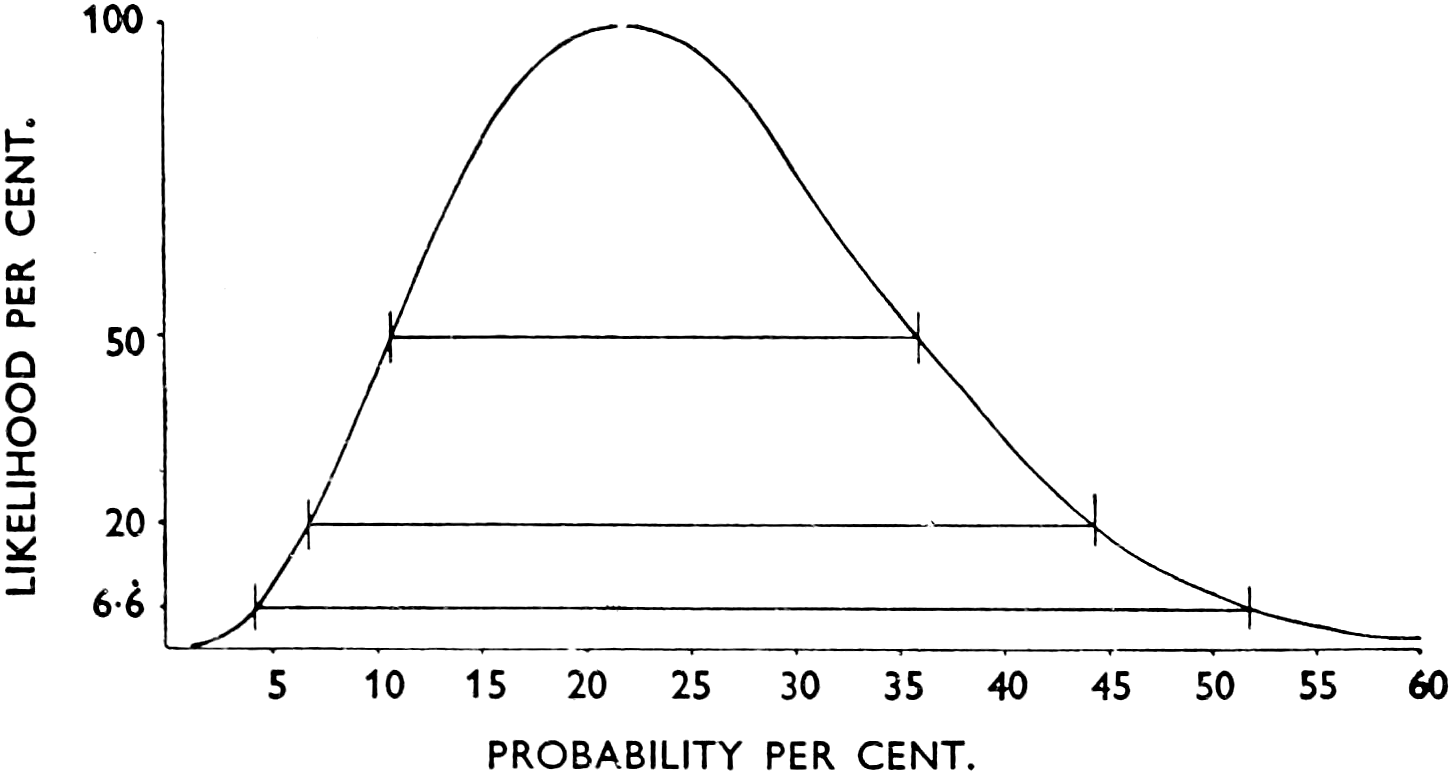
\includegraphics[width=0.95\textwidth]{figures/seacrhes_fisher_likelihood_binomial.png}
\caption[
Ratio thresholds of a Binomial likelihood function, reproduced from Fisher
]{%
Ratio thresholds of a Binomial likelihood function, reproduced from
Fisher~\cite{fisher1956statistical}.
Levels are drawn at $1/2$, $1/5$, and $1/15$ of its maximum.
Their extents could be reported in a table as a practical communication of
the likelihood function's profile.
}
\label{fig:searches_fisher_likelihood}
\end{figure}

\TODO{
Fisher:
``We can know nothing of the probability of hypotheses or hypothetical
quantities.
On the other hand we may ascertain the likelihood of hypotheses
and hypothetical quantities by calculation from observations''
~\cite{fisher1921probable}
Fisher:
``absurdly academic''
~\cite{fisher1956statistical}
% \begin{epigraphs}
% \qitem{%
% We can know nothing of the probability of hypotheses or hypothetical
% quantities.
% On the other hand we may ascertain the likelihood of hypotheses and
% hypothetical quantities by calculation from observations%
% }%
% {Ronald A. Fisher, 1921~\cite{fisher1921probable}}
% \end{epigraphs}
There is something horrifying in the ideological movement represented by the
doctrine that reasoning, properly speaking, cannot be applied to empirical data
to lead to inferences valid in the real world.
~\cite{fisher1956statistical}
}

\begin{singlespacing}
\begin{displayquote}
We can know nothing of the probability of hypotheses or hypothetical
quantities.
On the other hand we may ascertain the likelihood of hypotheses
and hypothetical quantities by calculation from observations
\end{displayquote}
\end{singlespacing}
~\cite{fisher1921probable}

\begin{singlespacing}
\begin{displayquote}
For all purposes, and more particularly for the \textit{communication} of the
relevant evidence supplied by a body of data, the values of the Mathematical
Likelihood are better fitted to analyse, summarize, and communicate
statistical evidence of types too weak to supply true probability statements
\end{displayquote}
\end{singlespacing}
~\cite{fisher1956statistical}

\begin{singlespacing}
\begin{displayquote}
There is something horrifying in the ideological movement represented by the
doctrine that reasoning, properly speaking, cannot be applied to empirical data
to lead to inferences valid in the real world.
\end{displayquote}
\end{singlespacing}
~\cite{fisher1956statistical}


\TODO{
Nayman-Pearson:
Seek good test statistics --
likelihood ratio intuitive for two-hypothesis comparison
prove it optimal in a reasonable sense
idea of long-run mostly not wrong
recede to maximum likelihood ratios
~\cite{neymanpearson1928max}
``for which hypothesis A is more probable and those for which it is less
probable (sic!)''
unbiased (unbiassed) test differs from unbiasedness of estimator
``Then the two corresponding densities at the sample point
are (Al) 6-42 x 10-20, (A2) 5 18*x 1O-4 and the ratio of the likelihood of Hypothesis
Al to- that of A2 is 1P24 x 10-16. This ratio confirms the common-sense judgment
that A2 is far more plausible than A1''
\^ Another posterior argument --- this likelihood ratio in in fact a change
in plausibilities. For example, if A2 is an inconsistent, self-contradictory
theory, it is totally implausible, and not more plausible despite predicting
these data better.
``The statistician can
balance the numerical verdict of likelihood against the vaguer expectations de-
rived from `a priori' considerations, and it must be left to his judgment to
at what point the evidence in favour of alternative hypotheses becomes so con-
vincing that Hypothesis A must be rejected.''
Introduce maximum likelihood ratio as interesting without claiming it to be
necessarily best.
Neyman-Pearson lemma --- reproduce Fig 5?
~\cite{neymanpearson19233lemma}
}

\begin{figure}[tp]
\centering
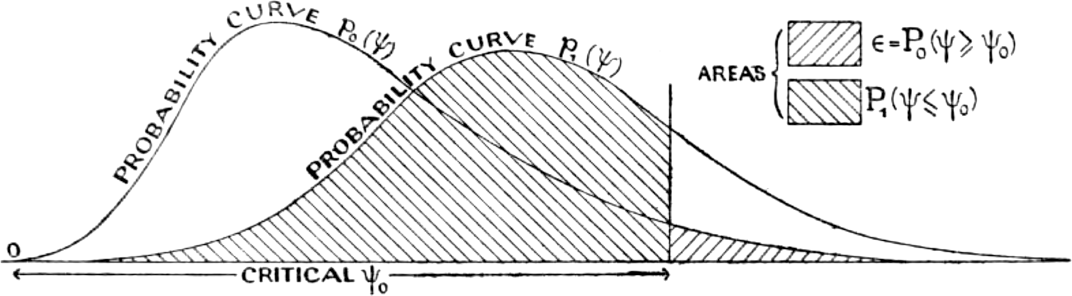
\includegraphics[width=0.95\textwidth]{figures/searches_np_curves_crop.png}
\caption[
Tail areas of prior data distributions from two alternative hypotheses,
reproduced from Neyman and Pearson
]{%
Tail areas of prior data distributions from two alternative hypotheses,
reproduced from Neyman and Pearson~\cite{neymanpearson19233lemma}.
}
\label{fig:searches_np_tails}
\end{figure}

Figure~\ref{fig:searches_np_tails}

\begin{figure}[tp]
\centering
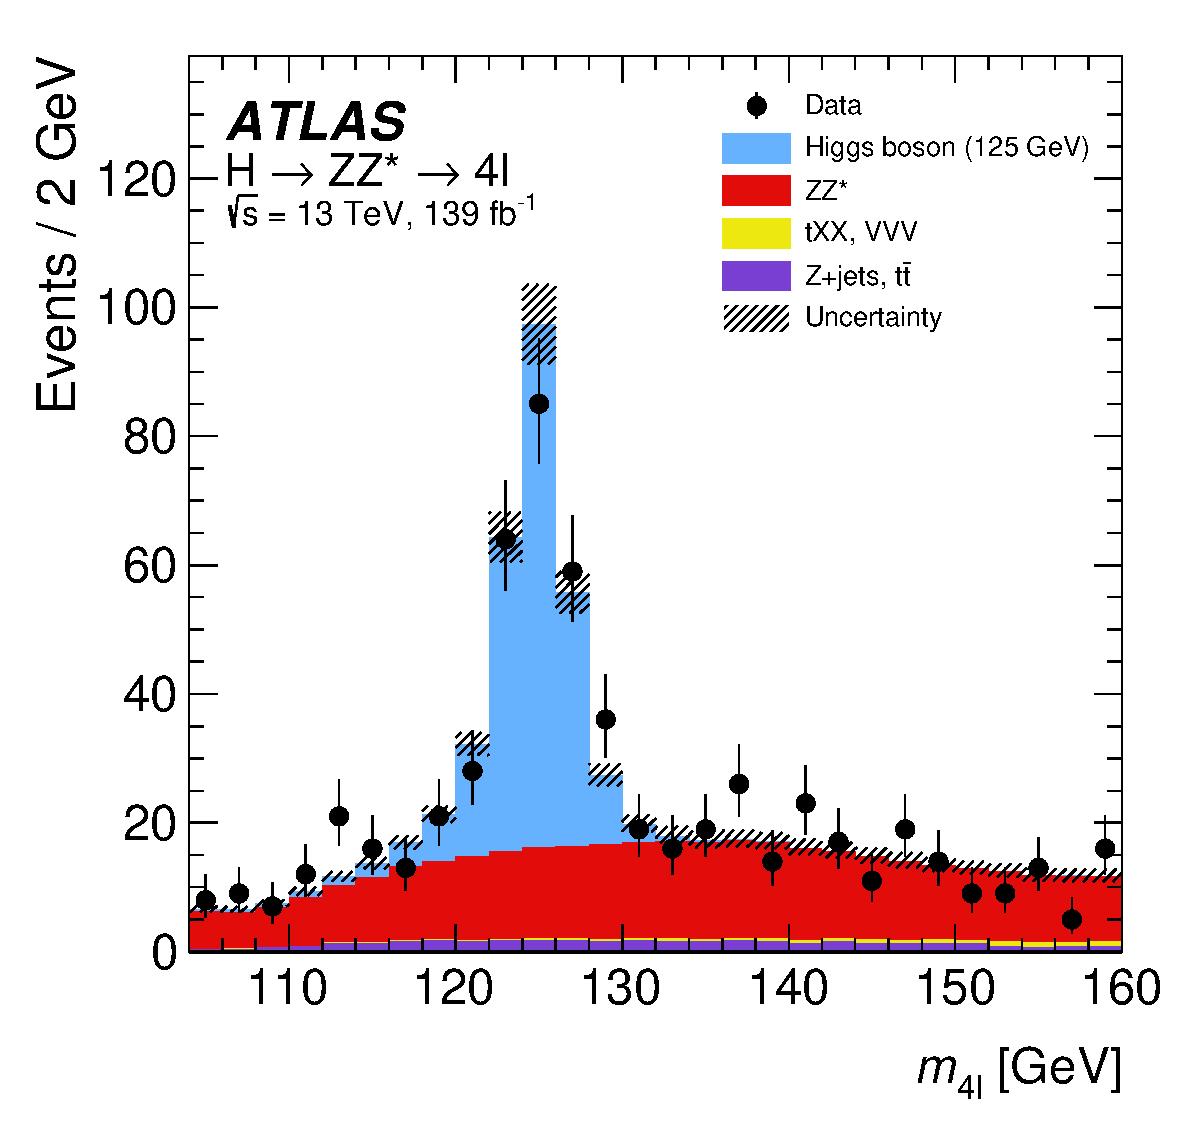
\includegraphics[width=0.6\textwidth]{figures/searches_atlas_higgs_4l_2207_00320.pdf}
\caption[
Signal and background distributions reproduced from the recent \atlas\
measurement of Higgs boson decays to $4\ell$
]{%
Signal and background distributions reproduced from the recent \atlas\
measurement of Higgs boson decays to $4\ell$~\cite{ATLAS:2022net}.
}
\label{fig:atlas_higgs_4l}
\end{figure}

Figure~\ref{fig:atlas_higgs_4l}

\TODO{
discrete failure to match --- randomization.
table of random numbers --- reputable table!
K. D. Tocher (1950)
``extraneous randomization''
~\cite{tocher1950discontinuous}
}

% TODO Kolmogorov axioms, unbiasedness
\TODO{
Given all this understanding, what I do not understand is their choice to
convert this to a $p$-value.
Seems to be this idea of long-run correctness guarantees.
But their derivation does rely on long-run frequencies.
}

\TODO{
restrict our notion of a probability with a special case: only frequency
of random events
}

\TODO{
tossing a coin is considered random
but if instead you are presented with a coin hidden under a cloth,
no frequency interpretation --- it either is or is not heads
you are therefore denied the ability to make uncertain predictions.
more generally, you are not allowed to express an uncertainty in something
unless some random process is involved
}

\TODO{
Can keep likelihoods, but cannot compute evidence values unless the prior
has a frequency interpretation.
}

\TODO{
Its void is filled with various proposed alternatives that do have frequency
interpretations and that sometimes yield useful results.
}

\TODO{
maximum likelihood, p-values, confidence intervals, and biasedness of
estimators.
}

\TODO{
Lehmann~\cite{lehmann2005testing};
p. 26 poisson inadmissable example;
L-unbiased with given loss function;
}


\TODO{maximum likelihood}
\TODO{p-value}
\TODO{p-value:
The chance of a small $p$-value is small.
This is true, but not interesting because the value of any $p$-value is small.
By construction $p$-values are uniformly distributed on the unit interval
under a given hypothesis.
The frequency of $p < 0.05$ is $5\%$, but so also is the frequency of
$0.6 < p < 0.65$.
The frequency of $p < \varepsilon$ is identical to the frequency
of $0.6 < p < 0.6 + \varepsilon$.
An appropriate choice of test statistic is therefore necessary for the
$p$-value to have meaning.
}
Figure~\ref{fig:searches_significant}
\TODO{confidence interval}
\TODO{unbiased}

\TODO{likelihood principle ~\cite{
birnbaum1962foundations,
savage1962foundations
}
}


\begin{figure}[tp]
\centering
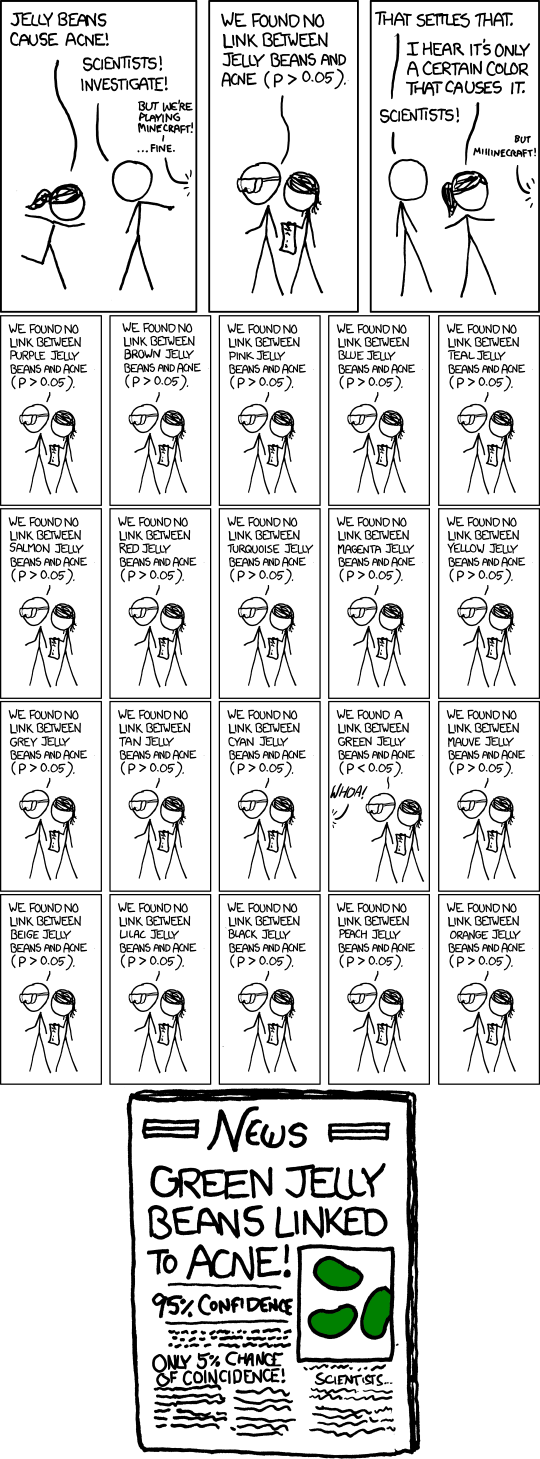
\includegraphics[width=0.46\textwidth]{figures/searches_significant_shrink.png}
\\
\begin{footnotesize}
`So, uh, we did the green study again and got no link. It was probably a{-}{-}'
\\
`RESEARCH CONFLICTED ON GREEN JELLY BEAN ACNE LINK; MORE~STUDY~RECOMMENDED!'
\end{footnotesize}
\caption[
``Significant'' by Randall~Munroe
]{%
``Significant'' by Randall~Munroe~\cite{xkcd2011significant}.
}
\label{fig:searches_significant}
\end{figure}


\begin{singlespacing}
\section{Post-frequentist practice}
\label{sec:searches_practice}
\begin{epigraphs}
\qitem{%
\ldots\ But this book, by its very excellence, its thoroughness, lucidity and
precision, intensifies my growing feeling that nevertheless the theory is
arbitrary, be it however ``objective,'' and the problems it solves, however
precisely it may solve them, are not even simplified theoretical counterparts
of the real problems to which it is applied.%
}%
{John~W.~Pratt,
\textit{Review: Testing Statistical Hypotheses},
1961~\cite{pratt1961testing}}
\end{epigraphs}
\end{singlespacing}


% significance measures
The ATLAS-recommended significance measure~\cite{atlas_significance} is
\begin{align}
\label{eqn:significance_atlas}
S_\mathrm{\atlas}(n; \mu, \sigma) =~&
\sqrt{2} \times
\mathrm{sign}(n - \mu) \times
\\[0.2em] \nonumber
&
\sqrt{
n\log\left(\frac{n(\mu + \sigma^2)}{\mu^2 + n\sigma^2}\right)
- \frac{\mu^2}{\sigma^2}\log\left(
1 + \frac{\sigma^2(n - \mu)}{\mu(\mu + \sigma^2)}
\right)
}
,
\end{align}
in an appropriate limit where $0\log(0x) = 0$ for the $n=0$ case.


\TODO{
on ``likelihood'' models ---
we are instructed to pretend that these are likelihoods on auxiliary data
TODO cite.
One is free to engage in such doublethink~\cite{orwell1949nnineteen},
% just as one is free to proclaim that $2 + 2 = 5$
but the fact remains that many constraints do not correspond to predictions of
auxiliary data so are not likelihoods: examples include
scale variations,
theoretical cross-section uncertainties,
non-closure uncertainties (which cover differences between estimates).
simulated sample comparisons,
statistical errors on weighted simulations,
extrapolation uncertainties,
and
all uncertainties on supersymmetric signal yields
(for which we have yet no data).
energy based modelling ---
I know of no tangible benefit from pretending that something is a likelihood
when it is not.
}

\section{Searches}
\label{sec:searches_searches}
% histograms, CR VR SR, systematics
% histfactory

\TODO{minimize energy not max logf}
To model the consequences of these many factors of uncertainty, each factor is
assigned a real-valued parameter, which when varied changed the expected yields
in the histogram bins of the search.
In this way, we form a statistical model which is a function
\begin{equation}
H_{\!f}(\vec \theta) \rightarrow (\vec \mu, \log f)
\end{equation}
from the parameters $\theta$ to Poisson expectations $\vec\mu$ of the histogram
bins and a regularization term $\log f$ that is maximized in fitting.

\histfactory~\cite{cranmer2012histfactory}
\pyhf~\cite{heinrich2021pyhf}
\histfitter~\cite{Besjes_2015,baak2015histfitter}


\clearpage

Hello again
